\documentclass[a4paper,14pt]{extarticle}

\newcounter{IsInsideAppendixToc}
\setcounter{IsInsideAppendixToc}{0}


\usepackage[T2A]{fontenc}
\usepackage[utf8]{inputenc}
\usepackage[english,russian]{babel}

\usepackage[newfloat]{minted}
\usepackage[dvipsnames]{xcolor}
\definecolor{aliceblue}{rgb}{0.94, 0.97, 1.0}
\usepackage{tikz-uml}
\usepackage[normalem]{ulem}
\usepackage{csquotes}


\usepackage[right=15mm, left=25mm, top=15mm, bottom=20mm, nohead]{geometry}

\usepackage{amsmath}
\usepackage{amsthm}
\usepackage{enumitem}
\usepackage{mathtools}
\usepackage{cmap}
\usepackage{array}
\usepackage{listings}

\renewcommand{\baselinestretch}{1.2}
\newtheorem*{definition}{Опр}

\DeclareMathOperator*{\VarInstr}{VarInstr}
\DeclareMathOperator*{\offset}{offset}

\usepackage{caption}
%\newenvironment{code}{\captionsetup{type=listing}}{}
\SetupFloatingEnvironment{listing}{name=Листинг}
\newenvironment{longlisting}{\captionsetup{type=listing}}{}

\usepackage{hyperref}
\usepackage{indentfirst}

\usepackage[
	backend=biber, %подключение пакета biber (тоже нужен)
	bibstyle=gost-numeric, %подключение одного из четырех главных стилей biblatex-gost 
	citestyle=numeric-comp, %подключение стиля стиля (а вот!) 
	language=auto, %указание сортировки языков
	babel=other, %указание языков
	sorting=ntvy, %тип сортировки в библиографии
	doi=false, 
	eprint=false, 
	isbn=false, 
	dashed=false, 
	url=false 
]{biblatex}
\addbibresource{library.bib}
\usepackage{bibentry}

\graphicspath{{img/}}
\usetikzlibrary{arrows.meta}
\usepackage{placeins}

%\DeclareFieldFormat{postnote}{#1} %убирает с. и p. 
%\renewcommand*{\multicitedelim}{\addsemicolon\space} % добавляет точку с запятой и пробел (; ) в перечислении
%\renewcommand*{\postnotedelim}{\addcolon\space}


\title{Разработка бэкенда LLVM для процессора CDM16}
\author{}
\date{}

% fix floats https://tex.stackexchange.com/questions/28556/how-to-place-a-float-at-the-top-of-a-floats-only-page
\makeatletter
\setlength{\@fptop}{0pt}
\setlength{\@fpbot}{0pt plus 1fil}
\makeatother


\usepackage{titletoc}

\usepackage{caption} %заголовки плавающих объектов

\captionsetup[figure]{name=Рисунок}
\DeclareCaptionLabelSeparator{longdash}{ -- }
\captionsetup{labelsep=longdash}




\begin{document}
	\begin{titlepage}
	\begin{center}	
		\footnotesize
		МИНИСТЕРСТВО ОБРАЗОВАНИЯ И НАУКИ РОССИЙСКОЙ ФЕДЕРАЦИИ 
		
		ФЕДЕРАЛЬНОЕ ГОСУДАРСТВЕННОЕ АВТОНОМНОЕ ОБРАЗОВАТЕЛЬНОЕ УЧРЕЖДЕНИЕ
		ВЫСШЕГО ОБРАЗОВАНИЯ
		
		«НОВОСИБИРСКИЙ НАЦИОНАЛЬНЫЙ ИССЛЕДОВАТЕЛЬСКИЙ ГОСУДАРСТВЕННЫЙ УНИВЕРСИТЕТ»
		
		(НОВОСИБИРСКИЙ ГОСУДАРСТВЕННЫЙ УНИВЕРСИТЕТ, НГУ)
		\vspace{0.25cm}
	\end{center}	
	\normalsize
	
	\noindent
	\begin{tabular}{l @{\hskip 1cm} l}
		Факультет &Информационных технологий \\
		Кафедра   &Систем информатики 
	\end{tabular}
	
	\vspace{0.5cm}
	
	\noindent
	\hskip 0.2cm Направление подготовки \hskip 0.3cm 09.03.01 Компьютерные науки и системотехника
	
	\vfill		
	
	\begin{center}
		\small	
		\textbf{ВЫПУСКНАЯ КВАЛИФИКАЦИОННАЯ РАБОТА БАКАЛАВРА}\\[4mm]
		\normalsize
		\uline{\hfill  Мерзляков Илья Алексеевич \hfill} 
		
		
		\normalsize
		Тема работы: 
		Разработка бэкенда LLVM для процессора CDM16
		%\bigskip		
	\end{center}
	\vfill
	
	\noindent
	\begin{tabular*}{\textwidth}{l @{\hskip 4cm} l}
		\textbf{\textquote{К защите допущен}}	& \textbf{Научный руководитель} \\
		& \\
		Заведующий кафедрой,		& б/с, доцент КафФТИ ФФ НГУ \\ 
		д.ф.-м.н., профессор		&  \\ 
		& \\
		\uline{Лаврентьев М.М.}/\uline{\hspace{2cm}} & \uline{Иртегов Д.В.}/\uline{\hspace{2cm}} \\ [-1.1ex]
		\scriptsize (фамилия, И.,О.) \hspace{0.5cm} (подпись, МП) & \scriptsize (фамилия, И.,О.) \hspace{0.5cm} (подпись, МП) \\
		& \\ 
		«...»...............20...г.& «...»...............20...г. 			
		
	\end{tabular*}
	\vfill
	\hfill
	\begin{minipage}{0.5\textwidth}
		Дата защиты: «...».............20...г.
	\end{minipage}
	
	\vfill
	
	\begin{center}
		Новосибирск, 2024 г.
	\end{center}
\end{titlepage}
	
	

\tableofcontents

\pagebreak
\section{Введение}

На ФИТ НГУ на курсе «Цифровые платформы» студентами изучается учебный 8-битный процессор CdM8. Из-за ограничений его архитектуры (8-битное адресное пространство, позволяющее использовать только 256 байт памяти), CdM8 не подходит для реализации на нем сложных проектов. В 2023 году группой студентов 3 курса ФИТ НГУ на основе этого процессора был разработан 16-битный процессор CdM16, имеющий 16-битное адресное пространство и позволяющий реализовывать более сложные проекты. Однако, написание кода на языке ассемблера – трудоемкая задача, значительно увеличивающая время разработки, а реализаций высокоуровневых языков для CdM16 в настоящий момент не существует.

В связи с этим было решено создать компилятор языка Си для процессора CdM16.

\pagebreak
\section{Обзор вариантов создания компилятора Си под новую архитектуру}

Есть два способа получить компилятор Си под новую архитектуру: разработать этот компилятор с нуля, или добавить поддержку новой архитектуры в уже существующий компилятор. Для выбора оптимального подхода сначала рассмотрим стадии компиляции программ на Си.

Процесс компиляции программ на языке Си состоит из нескольких этапов\cite{cpp_compilation}:
\begin{itemize}
	\item Препроцессинг - обработка директив препроцессора (начинаются с '\#');
	\item Компиляция - преобразование отдельных единиц трансляции в ассемблер целевой платформы;
	\item Ассемблирование - преобразование ассемблера в машинный код;
	\item Компоновка - связывание результатов компиляции отдельных единиц трансляции в единый исполняемый файл.
\end{itemize}

Последние два этапа уже реализованы авторами CdM16 в инструменте cocas, поэтому новому компилятору будет достаточно выполнять только препроцессинг и компиляцию. 

\subsection{Свой компилятор}

Компиляция программы на языке Си тоже состоит из нескольких этапов, и не все они зависят от целевой платформы:
препроцессинг, парсинг исходного кода, проверка типов и проведение некоторых оптимизаций производятся одинаково 
для всех архитектур, поэтому создание компилятора "с нуля" будет тратой ресурсов. 
Поэтому оптимальнее будет взять существующий компилятор, поддерживающий несколько архитектур, и добавить в него
поддержку CdM16.

\subsection{PPCI}

PPCI (Pure Python Compiler Infrastructure)\cite{ppci} - компилятор языка Си под различные архитектуры. Имеет бэкенды для архитектур 6500, arm, avr, m68k, microblaze, msp430, openrisc, risc-v, stm8, x86\_64 и xtensa, умеет компилировать языки C, Python, Pascal и Basic.   Попытка добавить в него поддержку CdM16 ранее предпринималась создателем CdM16 Николаем Репиным. Из-за низкого качества кода PPCI и отсутствия поддержки (проект не обновляется уже 3 года) попытка завершилась неудачей.

\subsection{LLVM/CLANG}
LLVM - это инфраструктура для создания компиляторов.  Архитектура LLVM достаточно модульная, в ней четко выделены части, отвечающие за парсинг входного языка (фронтенд) и генерацию машинного кода (бэкенд). В проект LLVM входит  clang, фронтенд для компиляции C и C++. Также фронтендами LLVM являются компиляторы языков rust и swift. LLVM написан на c++ (в отличие от GCC, написанного на C),что упрощает разработку новых бэкендов.

LLVM обладает обширной и подробной документацией, также про него написано множество статьей и книг, в том числе и про разработку бэкендов для него. При разработке своего бэкенда я, в основном, опирался на следующие источиники:
\begin{itemize}
	\item Writing an LLVM backend\cite{llvm:writing_backend} - статья из документации LLVM, в которой описана структура бэкенда и основные шаги для создания нового бэкенда;
	\item The LLVM Target-Independent Code Generator\cite{llvm:codegen} - статья из документации LLVM, в которой описан процесс генерации машинного кода целевой архитектуры;
	\item Building an LLVM Backend\cite{llvmleg} - доклад, в котором описаны основные шаги и трудности создания бэкенда на примере архитектуры leg;
	\item Creating an LLVM Backend for the Cpu0 Architecture\cite{cpu0} - книга о создании бэкенда для архитектуры cpu0. В этой книге достаточно подробно описано пошаговое создание бэкенда, также к книге приложены исходные коды бэкенда после каждой стадии разработки;
	\item Бэкенд LLVM для архитектуры Sparc\cite{llvm:sparc} - использован как пример.
\end{itemize}

Целевая архитектура в LLVM частично описывается на специальном декларативном языке tablegen, что сокращает объём кода, который необходимо написать для поддержки всех инструкций архитектуры\cite{llvm:codegen}.
\begin{figure}[h!]
	\begin{minted}[breaklines]{text}
def STWU  : DForm_1<37, (outs ptr_rc:$ea_res), (ins GPRC:$rS, memri:$dst),
	"stwu $rS, $dst", LdStStoreUpd, []>,
	RegConstraint<"$dst.reg = $ea_res">, NoEncode<"$ea_res">;
	\end{minted}
	\caption{Пример описания машинной инструкции в LLVM\cite{llvm:codegen}}
\end{figure}

Популярность  LLVM, его модульная архитектура и обилие литературы делают разработку бэкенда для него хорошим способом получить компилятор языка Си для новой архитектуры.


\subsection{GCC}
GCC (GNU Compiler Collection) - еще один открытый и популярный набор компиляторов. Также, как и LLVM, GCC также разделён на фронтенд и бэкенд, использует специальный язык для определения инструкций. Также GCC поддерживает 8- и 16-битные архитектуры.
\begin{figure}[h!]
	\begin{minted}[breaklines]{text}
(define_insn "tstsi"
	[(set (cc0)
	(match_operand:SI 0 "general_operand" "rm"))]
	""
	{
		if (TARGET_68020 || ! ADDRESS_REG_P (operands[0]))
		return "tstl %0";
		return "cmpl #0,%0";
	})
	\end{minted}
	\caption{Пример описания кода выбора инструкций в GCC\cite{gcc:codegen}}
\end{figure}
Все это делает GCC хорошим кандидатом для создания на основе него компилятора для CdM16, но по ряду причин, в том числе более современной, написанной на C++ кодовой базе LLVM ему было отдано предпочтение.

\pagebreak
\section{Обзор архитектуры LLVM}

Изначально проект LLVM создавался как фреймворк для компиляции и \emph{оптимизации программ во время исполнения} с помощью анализа во время выполнения и JIT-компиляции\cite{LLVM:CGO04}. В настоящее время LLVM используется и развивается как инфраструктура для AOT компиляции.
\begin{figure}[!h]
	\begin{center}
		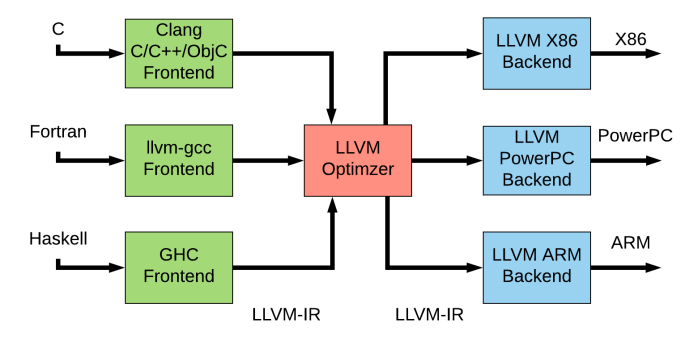
\includegraphics[width=\textwidth]{LLVM-Compiler-Development-architecture.png}
		\caption{Архитектура LLVM \cite{llvmpic}}
	\end{center}
\end{figure}

LLVM состоит из 3-х частей: фронтенда, транслирующего код на языке программирования в \emph{промежуточное представление} (IR)\cite{llvm:langref}, оптимизатора, производящего машинно-независимые оптимизации над IR, и бэкенда, транслирующего IR в инструкции целевой платформы. Так как фронтенд и оптимизатор не зависят от архитектуры, нам % кому нам я здесь одлин
понадобится разработать только бэкенд.

\subsection{LLVM IR}
LLVM IR - язык ассемблера, предназначенный для промежуточного представления программ между стадиями компиляции. IR является SSA (Static Single Assignment) языком, т.е. каждая переменная в нем присваивается только один раз. 
\begin{figure}[h!]
	\begin{minted}{c}
// Исходный код на Си
int example(int a, int b){
	if(a > b){
		return foo1(a, b);
	}else {
		return foo2(a, b);
	}
}
	\end{minted}
	
	\begin{minted}[breaklines]{llvm}
; Результат компиляции его в IR
define i16 @example(i16 noundef %a, i16 noundef %b)  #0 {
entry:
	%cmp = icmp sgt i16 %a, %b
	br i1 %cmp, label %if.then, label %if.else
if.then: 
	%call = tail call i16 @foo1(i16 noundef %a, i16 noundef %b) #2
	br label %return
if.else: 
	%call1 = tail call i16 @foo2(i16 noundef %a, i16 noundef %b) #2
	br label %return
return: 
	%retval.0 = phi i16 [ %call, %if.then ], [ %call1, %if.else ]
	ret i16 %retval.0
}
	\end{minted}
	\caption{Результат компиляции функции foo в IR}
	\label{ir_example}
\end{figure}

Пример кода на IR показан на листинге \ref{ir_example}. Как видно на примере, все значения присваиваются только один раз. При перезаписи переменных создаются новые переменные, а старые после перезаписи не используются. Этот подход работает только для функций, состоящих из одного базового блока (последовательности инструкций, имеющей одну точку входа, одну точку выхода, и не содержащей инструкций передачи управления ранее точки выхода \cite{contraol_flow_analysis}). В случаях, когда переменная зависит от прошлых итераций цикла или выполненной ветви условия  (как переменная \mintinline{llvm}|%retval.0| в примере ), используется инструкция phi - специальная инструкция, аргументами которой является пары базовый блок - значение, результатом этой инструкции является значение, соответствующее базовому блоку, из которого поток выполнения дошел до phi-ноды\cite{llvm:phi}.

\subsection{Tablegen}
Tablegen - специальный язык (DSL), используемый при разработке LLVM. Этот язык позволяет разрабатывать и обслуживать большое количество записей, специфичных для предметной области. На этом языке в LLVM описываются инструкции целевой платформы, соглашения о вызовах и классы регистров, также язык используется фронтендом Clang для объявления атрибутов. Сами по себе записи на tablegen ничего не значит, их смысл зависит от используемого tablegen-бэкенда. Например, из объявления инструкции tablegen-бэкендом gen-dag-isel генерируется C++ код, выбирающий эту инструкцию по паттерну инструкций IR, а бэкендом gen-asm-writer генерируется код, печатающий инструкцию в файл на языке ассемблера целевой архитектуры\cite{llvm:tablegen}.

\subsection{Архитектура бэкенда LLVM}
% https://llvm.org/docs/CodeGenerator.html#the-targetlowering-class
% https://llvm.org/docs/WritingAnLLVMBackend.html#instruction-relation-mapping

Бэкенд работает с IR в форме DAG (Direct Acyclic Graph) - графа, вершинами которого являются данные и инструкции, оперирующие  ими, а рёбрами - зависимость одних инструкций от результатов других. В основном вершины графа соответствуют инструкциям из IR, однако не весь IR автоматически представим в виде DAG. Некоторые инструкции, такие как вызов функций, получение их результата, получение значений параметров функции бэкенд должен 'спустить' (lower) в граф. Также не все инструкции и типы данных IR могут поддерживаться архитектурой (например, CdM16 не поддерживает 8-битные числа в регистрах), бэкенд должен 'легализовать' такие инструкции, т.е. заменить их несколькими поддерживаемыми инструкциями.

После построения DAG происходит \emph{выбор} (selection) инструкций, этим занимается \emph{SelectionDAG}. Инструкции целевой платформы описываются на специальном языке \emph{tablegen}. Tablegen позволяет компактно задать мнемонику инструкции, её входные и выходные регистры и шаблон (pattern) из вершин DAG, которому она соответствует. Большинство инструкций автоматически выбираются на основе шаблонов, однако некоторые нужно выбирать вручную.

После выбора инструкций бэкенд должен вывести их в текстовый ассемблерный файл. Части LLVM, ответственные за это, заточены под синтаксис GAS, который значительно отличается от ассемблера CdM16 \emph{cocas}, поэтому  необходимо изменить логику вывода ассемблерного кода, в частности, у cocas другой синтаксис меток,  другой синтаксис объявления секций, другие псевдоинструкции объявления констант,  ему необходимо указывать в начале файла импортируемые символы.


\pagebreak
\section{Обзор архитектуры CdM16}
CdM16 - это 16-битный Load-Store процессор, разработанный студентами НГУ для использования на курсе "Цифровые платформы"\cite{cdm:slides}. Основные технические характеристики:
\begin{itemize}
	\item 8 16-битных регистров общего назначения;
	\item Возможность адресовать 64 кБ адресного пространства;
	\item Арифметические инструкции принимают 3 операнда - 2 регистра-источника и регистр назначения.
\end{itemize}

\pagebreak
\section{Реализация бэкенда LLVM для CdM16}
\subsection{Описание архитектуры}
В первую очередь необходимо описать основные характеристики архитектуры: размеры типов данных и набор регистров. Первое описывается с помощью строки DataLayout. Для CdM16 эта строка выглядит так: \mint{text}|e-S16-p:16:16-i8:8-i16:16-m:C-n16|
Данный набор символов означает, что:
\begin{itemize}
	\item Платформа little-endian;
	\item Стек выровнен по 2 байта;
	\item Размер указателя - 2 байта;
	\item Переменные в памяти выравнивать не нужно;
	\item Платформа поддерживает арифметические операции только с 16-битными числами.
\end{itemize}

Набор регистров описан на языке tablegen в файле CDMRegisterInfo.td. У CdM16 8 регистров общего назначения, которые объединены в класс CPURegs:
\begin{minted}[breaklines]{text}
def CPURegs : RegisterClass<"CDM", [i16], 8, (add R0, R1, R2, R3, R4, R5, R6, FP)>;
\end{minted}
Объявление класса регистров необходимо для работы аллокатора регистров LLVM

\subsection{Описание инструкций}
Все инструкции CdM16 также описаны на tablegen и наследуются от класса CDMInst:
\mint[breaklines]{text}|class CDMInst<dag outs, dag ins, string asmstr, list<dag> pattern>: Instruction|

Параметры outs и ins определяют, какие регистры использует и изменяет инструкция; параметр instr\_asm задаёт мнемонику инструкции, параметр pattern задаёт шаблоны в SelectionDAG, которым соответствует инструкция. Большая часть инструкций наследуются от CDMInst не напрямую, а через другие классы.

Большинство арифметических инструкций наследуются от класса arithLogicR:
\begin{minted}[breaklines]{text}
class arithLogicR<string asm_instr, SDNode OpNode>:
  CDMInst<(outs CPURegs:$rd), (ins CPURegs:$rs0, CPURegs:$rs1),
    !strconcat(asm_instr, " $rs0, $rs1, $rd"),
    [(set CPURegs:$rd, (OpNode CPURegs:$rs0, CPURegs:$rs1))]>{
		// Некоторые параметры пропущены для краткости
}

def ADD: arithLogicR<"add", add>;
def SUB: arithLogicR<"sub", sub>;
// Также AND, OR, XOR
\end{minted}

Класс arithLogicR описывает инструкцию, имеющую два входных операнд-регистра и один выходной, и попадающую под шаблон "сохранить в регистр результат выполнения операции-параметра над входными регистрами". Инструкции, использующие этот класс, просто задают операцию для шаблону и мнемонику.

CdM16 также поддерживает инструкции сложения и вычитания с константой, они реализованы через класс arithLogicRi, в котором одним из параметров вместо регистра является immediate-значение (константа).

Битовые сдвиги в CdM16 не соответствуют битовым сдвигам в LLVM. Во-первых, в CdM16 нет инструкции сдвига на переменное кол-во бит, т.е. код \mintinline{c}|i << j| не скомпилируется. Эту проблему достаточно легко решить с помощью таблицы поиска, это будет сделано в новых версиях бэкенда. Также CdM16 может сдвигать не более, чем на восемь бит за раз. Эта проблема решается созданием мультикласса, добавляющего, в зависимости от константного аргумента, нужно ли добавлять дополнительную инструкцию сдвига:
\begin{minted}[breaklines]{text}
def imm1_8: ImmLeaf<i16, [{return (Imm >= 1) && (Imm <= 8);}]>;
def imm9_16: ImmLeaf<i16, [{return (Imm >= 9) && (Imm <= 16);}]>;
multiclass ShiftImm<string instr_asm, SDNode OpNode> {
 let Defs = [PSR] in {
	def _1_8 : CDMInst<(outs CPURegs:$rd), (ins CPURegs:$rs, shamt:$shamt),
	!strconcat(instr_asm, "\t$rs, $rd, $shamt"),
	[(set CPURegs:$rd, (OpNode CPURegs:$rs, imm1_8:$shamt))]>;
	
	def _9_16 : CDMInst<(outs CPURegs:$rd), (ins CPURegs:$rs, shamt:$shamt),
	!strconcat(
	!strconcat(instr_asm, "\t$rs, $rd, 8\n\t"),
	!strconcat(instr_asm, "\t$rd, $rd, $shamt-8")
	),
	[(set CPURegs:$rd, (OpNode CPURegs:$rs, imm9_16:$shamt))]>;
  }
}
defm SHL  : ShiftImm<"shl", shl>;
// And so on
\end{minted}

\subsection{Работа с памятью}
CdM16 имеет 3 основных способа адресации памяти:
\begin{itemize}
	\item Адрес в регистре;
	\item Адрес равен сумме двух регистров (полезно при доступе к элементам массивов и полям структур);
	\item Адрес равен сумме значения регистра FP и константы (полезно для доступа к переменным на стеке).
\end{itemize}

Выбор между режимами адресации реализован не через tablegen, а в файле CDMIselDAGToDAG.cpp. Инструкции для разнух способов адресации имеют разные паттерны адреса, LLVM выберет первую инструкцию, паттерн которой совпал с частью SelectionDAG. Второй режим выбирается, если адрес является суммой двух значений, иначе выбирается первый режим. Третий режим используется только для доступа к стеку.

\subsection{Стек и соглашение о вызовах}
CdM16 поддерживает адресацию относительно регистра FP (frame pointer, он же r7), поэтому для бэкенда он считается зарезервированным, в нем всегда хранится указатель на начало стекового кадра.
\begin{table}[!h]
	\begin{center}
		\begin{tabular}{ |c|c| }
			\hline
			Адрес & Содержимое \\
			\hline
			 & Предыдущий кадр \\
			 FP+2 & Адрес возврата \\
			 FP & Сохранённый FP \\
			 FP-2 .. SP & Локальные переменные \\
			 \hline
		\end{tabular}
		\caption{Структура стекового кадра (стек растёт вниз)}
	\end{center}
\end{table}

Каждая функция, использующая стек, имеет пролог и эпилог, создающие стековый кадр и восстанавливающие предыдущий:
\begin{minted}{asm}
# Пролог
pusр  fp # сохранить старое значение fp
ldsp  fp # загрузить в fp указатель на вершину стека
addsp N  # выделить на стеке N байт под локальные переменные
# Эпилог
addsp  N   # вернуть вершину стека обратно
pop    fp  # восстнанвить старое значение fp
\end{minted}

Соглашение о вызовах в данный момент позволяет передать до 4-х числовых параметров (в т.ч. указателей) в регистрах r0-r3, и возвращать одно числовое значение. Передача структур по значению и дополнительных числовых аргументов не поддерживается, но запланирована, она будет реализована записью на стек вызывающей функцией.

В данный момент существует ограничение на размер стекового кадра: максимальный оффсет относительно FP не должен превышать 64 байт для однобайтовых значение и 128 байт для двухбайтовых. Это связано с особенностью инструкций lsw, ssw и подобных им. В будущем для обхода ограничения при большом размере стекового кадра будут использоваться инструкции, адресующие память по сумме двух регистров.

\subsection{Вызов функций}

Поддержка вызова функций должна быть реализована в двух местах: при генерации кода вызывающей функции, и при генерации пролога и эпилога вызываемой функции.

Генерация кода вызова функции реализована в файле CDMISelLowering.cpp. Метод LowerCall генерирует код, размещающий аргументы в регистрах r0-r3, и на основании соглашения о вызовах определяет список регистров, которые должна сохранить вызывающая функция. Затем метод LowerCallResult вносит результат вызова в SelectionDAG функции (для текущего соглашения о вызовах это заключается в копировании данных из регистра r0).

Генерация обработки аргументов вызываемой функции также реализована в CDMISelLowering.cpp. Метод LowerFormalArguments вносит аргументы в SelectionDAG с помощью DAG.getCopyFromReg. Метод LowerReturn с помощью DAG.getCopyToReg помещает возвращаемое значение в регистр r0.

Методы SelectionDAG getCopyFromReg и getCopyToReg не всегда генерируют код, копирующий значения, они сообщают LLVM, что значение находится в определённом регистре или оно должно оказаться в определённом регистре.


\subsection{Инструкции условного перехода}

Условия оператора if и циклов компилируются в вершину BR\_CC\\SelectionDAG. У этой вершины аргументами являются condition code (код условия), два значения для сравнения и базовый блок, в который нужно перейти, если условие выполнено. Обработка условных переходов реализована в методе CDMDagToDagIsel::SelectConditionalBranch.
\begin{table}[!h]
	\begin{center}
		\begin{tabular}{ |l|l|l|  }
			\hline
			LLVM & CdM16 & Значение \\
			\hline
			SETLT & blt & < \\
			SETLE & ble & <= \\
			SETGT & bgt & > \\
			SETGE & bge & >= \\
			SETULT & blo & беззнаковое < \\
			SETULE & bls & беззнаковое <= \\
			SETUGT & bhi & беззнаковое > \\
			SETUGE & bhs & беззнаковое >= \\
			SETEQ & beq & ==\\
			SETNE & bne & != \\

			\hline
		\end{tabular}
		\caption{Соответствие кодов условия LLVM инструкциям условного перехода CdM16}
	\end{center}
\end{table}
Условный переход всегда раскрывается в последовательность инструкций cmp и b*. У такого подхода есть недостаток: из-за особенностей аллокатора регистров LLVM между любыми двумя инструкциями может быть вставлена инструкция move. Так как на CdM16 эта инструкция меняет флаги состояния процессора, устанавливаемые cmp, вставка её между cmp и b* некорректна. В данный момент в качестве временного решения вместо инструкции move используется макрос movens, раскрывающийся в последовательность push, pop. В будущем для решения этой проблемы планируется объединить инструкции cmp и b* в одну, чтобы LLVM не мог вставлять инструкции между ними.

\subsection{Оператор switch}

Оператор switch компилируется либо в несколько условных переходов, либо в таблицу поиска. Это делает clang/llvm. Для работы таблиц поиска потребовалось найти и исправить в коде LLVM место, где генерируются названия этих таблиц, так как ассемблер cocas не поддерживает (на момент написания) точку в названиях символов.

\subsection{Тернарный оператор}

Тернарный оператор и некоторые другие конструкции раскрываются LLVMом в вершины трех типов:
\begin{itemize}
	\item select - Выбрать одно из двух значений на основании boolean аргумента;
	\item setcc - Проверить условие на двух аргументах и вернуть boolean значение;
	\item select\_cc - setcc + select - проверить условие и выбрать одно из двух значений.
\end{itemize}

Так как в CdM16 отсутствуют conditional move инструкции, в которые удобно раскрывать select, и инструкции, в которые удобно раскрывать setcc, в бэкенде реализована обработка только select\_cc, а LLVM настроен автоматически раскрывать select и setcc в select\_cc. 

В методе CDMISelLowering::EmitInstrWithCustomInserter реализовано раскрытие select\_cc. Так как select\_cc раскрывается в уловный переход, выбрать его с помощью tablegen нельзя. Для раскрытия необходимо разделить базовый блок на две части, и добавить еще один. Переход из первой половины (HeadBB) во вторую (TailBB) напрямую происходит, если условие истинно, иначе происходит переход в дополнительный базовый блок (FalseBB), за которым следует TailBB. В HeadBB добавляется только инструкция сравнения и прыжка, в FalseBB ничего не добавляется, а в TailBB добавляется  $\phi$ инструкция. Инструкции move и безусловные переходы LLVM вставляет автоматически.

\begin{figure}[h!]
	\begin{center}
		\begin{tikzpicture}[
			squarednode/.style={rectangle, draw=black, very thick, minimum size=5mm,align=left},
			]
			\node[squarednode] (headbbnode) at (0, 0) {\textbf{HeadBB} \\ cmp r*, r* \\ b* TailBB };
			\node[squarednode] (falsebbnode) at (5, -3) {\textbf{FalseBB}};
			\node[squarednode] (tailbbnode) at (0, -6) {\textbf{TailBB} \\ phi(rTrue, HeadBB, rFalse, FalseBB)};
			
			\draw[-{Latex[length=5mm, width=2mm]}] (headbbnode.south) -- (falsebbnode.north);
			\draw[-{Latex[length=5mm, width=2mm]}] (headbbnode.south) -- (tailbbnode.north);
			\draw[-{Latex[length=5mm, width=2mm]}] (falsebbnode.south) -- (tailbbnode.north);
		\end{tikzpicture}
		\caption{Результат раскрытия select\_cc}
	\end{center}
\end{figure}

\begin{figure}[h!]
\begin{minted}{asm}
f:
# %bb.0: (HeadBB)
movens	r0, r1
ldi	r0, 1337
ldi	r2, 15
cmp	r1, r2
bgt	__LBB0_2
# %bb.1: (FalseBB)
ldi	r0, 228
__LBB0_2: # (TailBB)
rts
\end{minted}
\caption{Результат компиляции \mintinline{c}|int f(int a){return a > 15 ? 1337 : 228;}| }
\end{figure}

\subsection{Компоновка} 
За компоновку программ для CdM16 отвечает линкер, встроенный в ассемблер cocas.  Cocas, в отличие от GAS, требует явного указания внешних символов в начале секции. Для этого пришлось добавлять необходимы  функционал в классы LLVM AsmPrinter и MCAsmStreamer.

\subsection{Обработчики прерываний}
Функция-обработчик прерывания должна обладать следующими свойствами: вместо инструкции rts для возврата должна использоваться функция rti, все используемые регистры должны быть сохранены. Для создания таких функций было создано отдельное соглашение о вызовах. Список сохраняемых регистров задаётся через tablegen, выбор соглашения о вызовах для конкретной функции и выбор инструкции возврата реализуется на C++.
\begin{figure}[h!]
	\begin{minted}{text}
def CSR_O16_ALL : CalleeSavedRegs<(add FP,
(sequence "R%u", 0, 6))>;
	\end{minted}
	\caption{Список сохраняемых регистров для обработчиков прерываний}
\end{figure}

Для указания компилятору, какое соглашение о вызовах использовать, используются атрибуты. Их нужно добавлять не в бэкенд, а во фронтенд - компилятор clang. В результате был добавлен атрибут функций CDM\_ISR. При компиляции в IR clang для каждой функции определяет номер соглашения о вызовах, затем бэкенд в зависимости от этого номера выбирает инструкцию возврата (метод CDMInstrInfo::expandRet) и списки регистров, которые нужно сохранять (методы CDMRegisterInfo::getCalleeSavedRegs и\\ CDMRegisterInfo::getCallPreservedMask). Хотя в соглашении о вызовах указано, что необходимо сохранять все регистры, LLVM генерирует код, сохраняющий только используемые регистры. Если внутри обработчика прерывания вызывается другая функция, сохраняются все регистры, сохранность которых не гарантирована соглашением о вызовах вызываемой функции.
\begin{figure}[h!]
	\begin{minted}{c}
volatile int tick;
__attribute__((CDM_ISR))
void some_isr(){
	tick++;
}
	\end{minted}
	\caption{Пример обработчика прерываний}
\end{figure}

\clearpage
\section{Заключение}

В результате работы был создан компилятор языка Си для платформы CdM16, поддерживающий значительное подмножество возможностей языка Си: создание функций, принимающий до 4 числовых аргументов, 8- и 16-битные переменные, циклы, ветвления, структуры, массивы, глобальные переменные, статические и внешние символы.

Пример проекта, написанного на Си под CdM16 - \href{https://github.com/leadpogrommer/llvm-project-cdm/tree/backend/cdm/llvm/test_cdm/life_multifile}{реализация игры "жизнь"}.

В настоящий момент компилятор уже используется авторами CdM16 для разработки операционной системы для компьютера, основанного на CdM16\cite{cdm:coconut}, также как минимум 2 команды студентов курса "Цифровые Платформы"\allowbreak используют компилятор для создания проектов.

\subsection{Планы на будущее}

В будущем планируется реализовать:
\begin{itemize}
	\item Программную реализацию 32-битной арифметики;
	\item Поддержку передачи аргументов на стеке;
	\item Поддержку функций с переменным количеством аргументов (vararg);
	\item Минимальную стандартную библиотеку Си;
	\item Покрыть бэкенд тестами.
\end{itemize}


\pagebreak
\printbibliography
\addcontentsline{toc}{section}{\refname}


\newpage
\begin{center}
	\textbf{\large ПРИЛОЖЕНИЕ А}
\end{center}
\refstepcounter{section}
\addcontentsline{toc}{section}{ПРИЛОЖЕНИЕ А}
\vspace*{\fill}
	\begin{center}
		\textbf{\large КОМПИЛЯТОР CLANG ДЛЯ ПРОЦЕССОРА CDM16\\РУКОВОДСТВО ПОЛЬЗОВАТЕЛЯ}
	\end{center}
\vspace*{\fill}
\newpage
\setcounter{section}{0}
%\addtocontents{toc}{\protect\setcounter{tocdepth}{-2}}


% Я не ебу, как и почему оно работает
\setcounter{IsInsideAppendixToc}{1}
\addtocontents{toc}{\protect\setcounter{tocdepth}{\value{IsInsideAppendixToc}}}

\textbf{\Large Содержание}


\startcontents[chapters]
\printcontents[chapters]{}{0}[4]{}

\pagebreak
\section{Аннотация}
В данном документе приведено руководство оператора по применению и эксплуатации компилятора clang для процессора CdM16. В данном документе, в разделе «Назначение программы» указаны сведения о назначении программы и информация, о функциональности программы и ее эксплуатации. В разделе «Условия выполнения программы» перечислены условия, являющиеся необходимыми для выполнения программы. Раздел «Выполнение программы» содержит действия оператора, необходимые для загрузки, запуска, выполнения и завершения программы. В разделе «Сообщения оператору» приведены тексты сообщений, выдаваемых в ходе выполнения программы, описание их содержания и соответствующие действия оператора (действия оператора в случае сбоя, возможности повторного запуска программы и т.п.).

Оформление программного документа «Руководство оператора» произведено по требованиям ГОСТ 19.505-79 «ЕСПД. Руководство оператора».

\newpage 
\section{Назначение программы}
\subsection{Функциональное назначение}
Программный продукт предоставляет возможность компилировать программы, написанные на подмножестве языка Си, в язык ассемблера CdM16.
\subsection{Эксплуатационное назначение}
Программа может применяться студентами первого курса нового потока ФИТ НГУ для реализации проектов в рамках курса “Цифровые платформы”. Также программа подходит студентам старших курсов, разрабатывающим ПО для платформы CdM16.
\section{Получение программы}
Скомпилированную для ОС Windows программу можно скачать по ссылке: \href{https://drive.google.com/drive/folders/1_hNkdGcA6mFwb-5KPrtYAG46lwwvFffL}{https://drive.google.com/drive/folders/1\_hNkdGcA6mFwb-5KPrtYAG46lwwvFffL}. Для других операционных систем необходимо собрать программу из исходного кода.

Для сборки необходим компьютер с OS Linux или macOS, а также с git, gcc/clang и ninja. Чтобы собрать программу, выполните следующие шаги:
\begin{minted}[breaklines]{shell}
# склонируйте репозиторий
git clone --depth=1 --branch=backend/cdm https://github.com/leadpogrommer/llvm-project-cdm.git
# создайте папку сборки
mkdir llvm-project-cdm/llvm/build && cd llvm-project-cdm/llvm/build
# сконфигурируйте проект
cmake -G Ninja  -DLLVM_ENABLE_PROJECTS=clang -DLLVM_TARGETS_TO_BUILD= -DLLVM_PARALLEL_LINK_JOBS=6 -DLLVM_USE_LINKER=lld -DLLVM_EXPERIMENTAL_TARGETS_TO_BUILD=CDM -DCMAKE_BUILD_TYPE=Release ..
# соберите проект
cmake --build .
# проверьте работу компилятора
bin/clang -print-targets 
\end{minted}

\section{Условия выполнения программы}
Для работы программы требуется компьютер под управлением операционной системы GNU/Linux, Windows или macOS, отвечающий минимальным системным требованиям используемой операционной системы.
\section{Выполнение программы}
Запуск программы производится из командной строки. Формат аргументов следующий:
\mint{text}|./clang -target cdm -S -O1 <<source_file>> -o <<output_file>>|
где \mintinline{text}|<<source_file>>| - путь к файлу с исходным кодом на языке Си, \mintinline{text}|<<output_file>>| - путь к файлу, в который будет сохранен результат компиляции.
\section{Входные данные}
Входные данные должны быть синтаксически корректной программой на языке Си. В данный момент не все возможности языка Си поддерживаются, основными ограничениями являются:
\begin{itemize}
\item Невозможность передавать больше 4-х аргументов в функцию;
\item Невозможность передавать в функции и возвращать из функций структуры по значению;
\item Невозможность побитово сдвигать на переменную величину (1 << j);
\item Отсутствие поддержки длинной арифметики (int32\_t, int64\_t) и арифметики с плавающей точкой.
\end{itemize}
\section{Выходные данные}
Результатом работы программы является текстовый файл с кодом на языке ассемблера CdM16. Для сборки результата в бинарный машинный код необходимо использовать ассемблер cocas.
\section{Сообщения оператору}
В случае возникновения ошибки программа выводит информацию о ней в стандартный поток ошибок (stderr)


\end{document}